%%%%%%%%%%%%%%%%%%%%%%%%%%%%%%%%%%%%%%%%%%%%%%%%%%%%%%%%%%%%%%%%%%%%%%%%%%%%%%%%
%2345678901234567890123456789012345678901234567890123456789012345678901234567890
%        1         2         3         4         5         6         7         8

\documentclass[letterpaper, 10 pt, conference]{ieeeconf}  % Comment this line out
                                                          % if you need a4paper
%\documentclass[a4paper, 10pt, conference]{ieeeconf}      % Use this line for a4
                                                          % paper

\IEEEoverridecommandlockouts                              % This command is only
                                                          % needed if you want to
                                                          % use the \thanks command
\overrideIEEEmargins
% See the \addtolength command later in the file to balance the column lengths
% on the last page of the document

\pdfminorversion=4

% The following packages can be found on http:\\www.ctan.org
%\usepackage{graphics} % for pdf, bitmapped graphics files
%\usepackage{epsfig} % for postscript graphics files
%\usepackage{mathptmx} % assumes new font selection scheme installed
%\usepackage{times} % assumes new font selection scheme installed
%\usepackage{amsmath} % assumes amsmath package installed
%\usepackage{amssymb}  % assumes amsmath package installed
\usepackage{amsmath}    			% ams packages for mathematics environment    
\usepackage{amssymb}
\usepackage{amsfonts}
%\usepackage{amsthm}

\usepackage{graphicx}  				% Versatile graphics manipulation options

\usepackage[croatian]{babel}  % Croatian typographical rules and hyphenation patterns 
\usepackage[utf8]{inputenc}  	% Encoding of Croatian characters
\usepackage[T1]{fontenc}
\usepackage{ae,aecompl}     	% Type 1 fonts, similar to Computer Modern

\usepackage{microtype}				% Improves spacing

\usepackage{subfig}

\usepackage{tabularx}
\usepackage{booktabs}
%\newcolumntype{C}{>{\centering\arraybackslash}X} % centered version of "X" type
\setlength{\extrarowheight}{1pt}
\usepackage{enumerate}				% Additional options for listing of items in enumerate environment
\usepackage{algorithm2e}			% Writing pseudo-code
\usepackage{todonotes}				% Adding todo items
\usepackage{dirtree}					% Simple display of directory tree
\usepackage{hyperref}					% Managing cross-referencing


\usepackage{lmodern}
\usepackage{nccmath}
\usepackage{mathptmx}
\usepackage[keeplastbox]{flushend}
\usepackage{scalerel,stackengine}
\DeclareMathOperator*{\argmax}{argmax} % thin space, limits underneath in displays
\DeclareMathOperator*{\argmin}{argmin}
\stackMath
\newcommand\reallywidehat[1]{%
	\savestack{\tmpbox}{\stretchto{%
			\scaleto{%
				\scalerel*[\widthof{\ensuremath{#1}}]{\kern.1pt\mathchar"0362\kern.1pt}%
				{\rule{0ex}{\textheight}}%WIDTH-LIMITED CIRCUMFLEX
			}{\textheight}% 
		}{2.4ex}}%
	\stackon[-6.9pt]{#1}{\tmpbox}%
}
\parskip 1ex

%calligraphy packages
\usepackage{calrsfs}
\DeclareMathAlphabet{\pazocal}{OMS}{zplm}{m}{n}
\newcommand{\Ca}{\pazocal{C}}
\newcommand{\Oa}{\pazocal{O}}
\newcommand{\Va}{\pazocal{V}}
\newcommand{\Ua}{\pazocal{U}}
\newcommand{\Aa}{\pazocal{A}}
\newcommand{\Ta}{\pazocal{T}}
\newcommand{\La}{\pazocal{L}}
\newcommand{\tp}[1] {\todo[inline, color=green]{MK: #1}}
\newcommand{\Ja}{\pazocal{J}}

\graphicspath{{./figures/}}
\usepackage{float}

\providecommand{\indexterms}[1]{\textbf{\textit{Index terms---}} #1}

\title{\LARGE \bf
	A Survey on Multi-Robot Autonomous Coordinated Exploration Strategies
}
\author{Ana Batinovi\'{c} \\
	University of Zagreb, Faculty of Electrical Engineering and Computing \\
	Department of Control and Computer Engineering\\
	Laboratory for Robotics and Intelligent Control Systems (LARICS) \\
	Unska 3, 10000 Zagreb \\
	Email: ana.batinovic@fer.hr
}

\makeatletter
\newcommand{\removelatexerror}{\let\@latex@error\@gobble}
\newcommand{\mb}[1]{\boldsymbol{#1}}
\newcommand{\norm}[1]{\left\lVert#1\right\rVert}

\makeatother

\begin{document}
\maketitle

\thispagestyle{empty}
\pagestyle{empty}


%%%%%%%%%%%%%%%%%%%%%%%%%%%%%%%%%%%%%%%%%%%%%%%%%%%%%%%%%%%%%%%%%%%%%%%%%%%%%%%%
\begin{abstract}

This paper proposes a short overview of multi-robot exploration strategies of an unknown environment. The main idea of the exploration strategy is an appropriate region selection as well as the minimization of a cost function involving the distance traveled by the robots, the time it takes for them to finish the exploration, and others. The paper focuses on multi-robot systems that could accomplish an unknown area exploration under required conditions.
These strategies play an important role in 2D as well as in 3D spaces. Therefore, this paper presents a systematic survey on the existing literature on coordination and exploration in the both spaces. The paper describes our recent work in autonomous multi-robot exploration systems and mapping using decentralized approach.
A brief conclusion and further research perspectives are given at the end of the paper. 

 
\indexterms{Multi-Robot System, Target Point, Exploration, Mapping, Frontiers, OctoMap.}

\end{abstract}
\section{introduction}

Application of multi-robot systems to solving core robotics problems has drawn significant attention in the last few decades. One example is coordination of a robot team for exploration of an unknown area, which is encountered in many applications, such as search and rescue (\cite{Murphy2004}), cleaning (\cite{Endres}), (\cite{Pinheiro2015}), warehousing (\cite{Wurman2008}) or planetary exploration (\cite{Mataric2001}), to name a few. Due to the fact that autonomous multi-robot systems are entering society and as such will interact with people on a daily basis, development of efficient coordination algorithms becomes necessary.

Robots need a map in order to operate in a particular environment. The ability of robots to autonomously travel around an unknown environment gathering the necessary information to obtain a useful map for navigation is called autonomous exploration \cite{Julia2012}. 

Like in the human society, robots can be more effective when they work together. Moreover, a robot team can accomplish a predefined task much quicker than a single robot can (\cite{Dias2000}). Another advantage of robot teams is the possibility of sensor fusion, which in turn can help to compensate for sensor uncertainty (\cite{Wurm2008}).
If done properly, multi-robot coordination can lead to i) task accomplishment in shorter time, ii) increased robustness, iii) higher map quality, and finally iv) the completion of tasks impossible to be performed by a single robot (\cite{Dias2006}).

This paper focuses on different exploration strategies using a multi-robot system with coordinated robots that could accomplish a given task in a way which minimizes the overall exploration time. These strategies play an important role in 2D as well as in 3D spaces. Therefore, this paper makes an extensive overview of the exploration strategies in both spaces. This paper also presents our 2D decentralized exploration strategy using multiple robots as well as 3D autonomous building exploration solution with purpose of fire detection.

The rest of the paper is organized as follows. 
In Section II an overview of 2D exploration strategies is given. Section III briefly describes existing 3D exploration strategies, and in the final section a conclusion and future work are given.

\section{2d exploration strategies}
\tp{Ovdje bi bilo dobro staviti uvodnih par recenica koje ce se opisati u par recenica 2D exploration tj. da imamo vise robota koji imaju (nesavrsene) senzore, explored i unexplored space, donosimo odluku tocno gdje cemo ici u smjeru unexplored prostora. Reci da robot treba znati sto tocnije svoju poziciju sto tocnije. Mozes se i samo referencirati na postojecu Fig. 1 ili dodati novu. Mozes i navesti u kojem formatu zelimo dobiti mapu i koji se senzori najcesce koriste.
}
\tp{Također bi trebalo slikovito prikazati strukturu rjesenja (nesto kao Fig 3., ali malo opcenitije). Ovo mozes za prezentaciju, ne trebas sad.}

Exploration algorithms can be grouped into centralized and decentralized. In \st{the}  centralized approaches, each robot receives tasks from a single central \emph{leader}, which runs the overall planning algorithm, and afterwards the robot sends its info back to the leader. {\color{red}A} centralized assignment may be less practical due to communication limits (\cite{Dias2000}), robustness issues (\cite{Dias2006}), or {\color{red}the} time required for algorithm execution and scalability (\cite{Julia2012}). An advantage of centralized approaches is that optimal plans can be found (\cite{Yan2011}). For instance, Sharma et al. \cite{SharmaHonc2016} used a centralized exploration \st{approach} {\color{red}strategy} based on routing priority. The algorithm keeps track of the frontiers, assigning them to robots whenever they fall into {\color{green}a trap situation}.

\tp{Sto je trap situation, mozda bolje koristiti neki drugi izraz}

In contrast to centralized approaches, in a decentralized approach, the robots are completely ({\color{red} or at least partially}) independent throughout the exploration process. Each robot has its own local knowledge of the world and can decide its future actions by taking into account its current context and tasks, its own capacities and the capacities of the other robots. \st{through a negotiation process} (\cite{Yan2013}) {\color{red} Robot send and received information to/from other robots in its communication range}. Moreover, it typically has better reliability, flexibility, adaptability and robustness (\cite{Zlot2002}). 
 
There are several representative approaches from \st{the} both centralized and decentralized 2D exploration strategies described in the following text. 

\subsection{Nearest Frontier Approach} 
An unexplored area is usually represented using an occupancy grid map introduced by \cite{Moravec}. While a robot moves, an occupancy likelihood for each cell of the grid is updated with the information \st{of} {\color{red} gathered by} sensors. Depending on this occupancy likelihood, cells can be classified as free, occupied or unknown (Fig. \ref{fig:environment}). Using an occupancy grid, a robot can reach an unexplored zone navigating to the frontier cells that separate the free cells from the unknown cells known as \textit{frontiers} \cite{Yamauchi1997}. A general frontier exploration diagram is shown in Fig. \ref{fig:flow_diagram}.
\begin{figure}[t!]
	\centering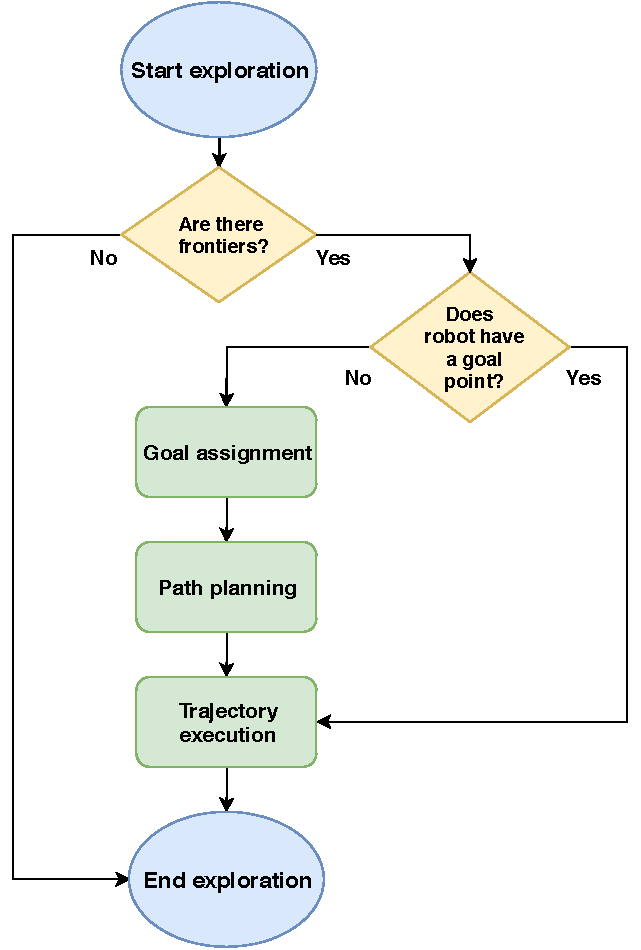
\includegraphics[width=0.85\columnwidth]{./pictures/flow_diagram.pdf}
	\caption{Flow diagram for the frontier exploration strategies. \In case a robot {\color{red}is idle} (does not have a goal point), a new goal is computed, assigned, a path to the assigned goal is obtained and a trajectory executed.}
	\label{fig:flow_diagram}
\end{figure}
Yamauchi's technique consists in selecting the shortest path to the nearest frontier. In this way, the target cell selected by this technique $t_{NF}$ is:
\begin{equation}
t_{NF} = \argmin_{a \in F} L(a), 
\label{equation:t-nf}
\end{equation}
where $L(a)$ represents the length of the shortest path to reach the cell $a$ ($a_{i}$, $a_{j}$) and $F$ the subset of the frontier cells \cite{Julia2012}. As it can be noticed, (\ref{equation:t-nf}) takes into account the cost of reaching a frontier cell and does not provide any coordination mechanism. In case a single robot system is extended to a multi-robot system, robots may select the same frontier if they are situated in nearby positions. For instance, \cite{Yamauchi1998} extended his nearest frontier approach to multiple robots using global maps built by each robot with the information provided by all robots. Since robots share the acquired information, exploration is cooperative, \st{but robot movements are uncoordinated} {\color{red}however, the selection of target points remains uncoordinated}. When the robots are in \st{close positions} {\color{red}the vicinity of each other} it is likely that they {\color{red}are going to} choose the same frontier {\color{red}point or region} to explore if no other coordination mechanisms are considered.

Frontier exploration strategies are also extended to a multi-robot system in \cite{Simmons2000} and \cite{Burgard2005}. Simmons \cite{Simmons2000} used a semi-distributed model where a centralized module integrates local data from a team of robots. The team used a probabilistic technique to build a global map in a coordinated fashion. \st{Due to the problem of absolute positioning techniques in indoor environments, robots must estimate their local pose in an environment, leading to odometry errors.} {\color{red}To account for odometry errors in determination of absolute robot position}, Simmons used probability calculations to estimate the local pose of each robot, and built a global map by joining each individual robots local map. 
While Simmons \cite{Simmons2000} implements coordination between robots by sharing of map information and reducing the utility of frontier points in the vicinity of an allotted point, Burgard \cite{Burgard2005} came up with an elegant bidding process. 

A dense frontier points detection method implemented by Orsulic (\cite{Orsulic2019}) is an extension to Google Cartographer (\cite{Hess2016}) that has achieved good results in terms of wall-time per frontier update, which greatly speeds up {\color{red}the} exploration process. Orsulic used nearest frontier approach in order to explore an area. 

Rekeleitis \cite{Rekeleitis2000} covered terrains with multiple robots where at least one robot was stationary and posed as an observer. In \cite{Fox2006} a decision theoretic approach to multi-robot exploration was presented where the main problem was to decide whether a robot should explore the terrain or \st{to} verify the hypothesis of other robots whose states are not mapped into a common reference frame. The nearest unexplored region technique is also used by Wullschleger \cite{Wullschleger99}, Santosh \cite{Santosh2008}, Murphy and Newman \cite{Murphy2008}, to name a few \st{more}.

\subsection{Cost-Utility Approach}
Generally, in a cost-utility approach a goal point maximizes the benefit {\color{red}(difference)} between utility and cost. The utility is {\color{red}calculated as the expected information gain from visiting the position of the goal point} \st{measured in terms of the expectation of the information incorporated to the occupancy map from the position of the goal point}. An example of cost-utility approach was presented by González-Baños and Latombe \cite{GonzlezBaos2002}. Frontier cells are designated as candidate destinations and the benefit $B_{CU}(a)$ to reach a candidate cell a is evaluated according to the following expression:
\begin{equation}
B_{CU}(a) = U(a) - \lambda_{CU}C(a),
\label{equation:cost-utility}
\end{equation}
where $U(a)$ is a utility function, $C(a)$ is a cost function and $\lambda_{CU}$ is a constant that adjusts the relative importance between both factors \cite{Julia2012}. Utility and cost functions are expressions normalized in the range $\left[0, 1\right]$ that are calculated as follows:
\begin{equation}
U(a) = \frac{U_{nex}(a, R_{s})}{\pi R_{s}^{2}},
\end{equation}
\begin{equation}
C(a) = \frac{L(a)}{max_{b \in F}L(b)},
\end{equation}
where the function $U_{nex}(a, R_{s})$ is \st{the result of counting} the number of unexplored cells in the range of the sensor from cell $d$ {\color{green}cell $a$?}, \st{being} $R_{s}$ {\color{red}being} the maximum range of the sensor expressed in cell units.
Then, the target cell $t_{CU}$ is chosen as the one that maximizes the utility-cost relation \cite{Julia2012}:
\begin{equation}
t_{CU} = \argmax_{a \in F} B_{CU}(a).
\end{equation}
Similar to the work proposed by Simmons, Burgard \cite{Burgard2000} introduced \st{some} coordination by means of reducing \st{a determined initial utility given to each frontier depending on the likelihood of being in the sensor range from other frontiers that have been assigned to other robots.} {\color{red} the utility of a frontier point depending on the likelihood that it is in the vicinity of a frontier point already-assigned to another robot.} The assignment of frontiers to robots is made {\color{red}in a greedy manner} (sequentially) using a cost-utility approach with the length of the minimum path {\color{red}{to a frontier point}} as cost. It is assumed that robots know each others relative positions. {\color{green}The algorithm determines optimal target points for each robot that increase the coverage by the maximum amount at that time period - Ovo je nejasno napisano, napisi tocno sto se odvija, npr. In each iteration of the assignment algorithm, the best robot-to point assignment is calculated using cost-utility. The chosen robot is not considered in the next iteration - ne znam tocno kako ide.}. Moreover, Burgard in \cite{Burgard2005} suggested that the assignment of frontiers to robots could be optimized using the Hungarian method \cite{Kuhn1955} instead of the sequential assignment.

Another example of cost-utility model is given in \cite{Umari2017}, where a frontier detection method is based on Rapidly Exploring Random Trees (RRTs). Umari defines revenue from a frontier point as a combination of an information gain and navigation cost. 
 
Bhattacharya et al. \cite{Bhattacharya2013}, \cite{BhattacharyaGhrist2013} focused on the use of cost functions related to information theory, casting the exploration problem as a minimization of map entropy. Authors combined this approach with a grid-based map decomposition with an entropy minimization which results in complete coverage of a known map and full exploration if the scenario is unknown. 

\subsection{Market-Based Approach}
\tp{Po meni su ovo sve cost-utility problemi, a onda se dalje dijele na 1)Greedy/simple 2)Market-based 3) Optimization based - jesam li u krivu?}

The general concept of the market-based approaches includes independence of robots in terms of planning, and the ability of robots to take team resources into account.
Relatively close to Burgard's approach in \cite{Burgard2000}, Zlot \cite{Zlot2002} uses a market architecture for the multi-robot mapping and exploration problem that aims to minimize an overall exploration time. In market-based coordinated approach each robot contains a list of goal points and \st{profits} {\color{red}benefits} associated with (\ref{equation:cost-utility}). Each robot selects the most profitable target as destination and when after reaching a current goal point, a robot initiates an auction. For each point in auction, each robot makes a bid with its current profit aiming to minimize own travel distance and maximize new area information.

It is shown in \cite{Dias2003} when different team sizes are included, a market method has an advantage over a centralized approach in terms of travelled distance. 

Michael et al. \cite{Michael2008} proposed a marked-based coordination protocol where robots are able to bid for task assignment with the assumption that every robot has knowledge of the maximum number of robots that any given task can accommodate. Each auction is performed among neighboring groups of robots and requires only local communication.

Sheng et al. \cite{Sheng2006} proposed an algorithm based on a distributed bidding model to coordinate the movement of multiple robots with limited communication range. The bidding algorithm takes into consideration distances between robots and a map synchronization mechanism reduces the exchanged data volume when robot subnetworks merge.

\subsection{Decentralized Coordinated Approach}

Pereira et al. \cite{Pereira2015} proposed a new exploration and mapping strategy, which relies on individual decision rules and communication of topological maps to achieve efficient and fast mapping. In this distributed strategy each robot broadcasts a graph representing the topological map, which can be transmitted to robots that are not within the communication range (through other robots in a system). 

Decentralized coordinated approach described in \cite{Colares2016} showed how exploration efficiency can be greatly improved. Authors presented a decentralized approach for multi-robot exploration that leverages the classical frontier based methods. The strategy took into consideration a utility function (the information gain) and the distance costs of frontiers. In that manner, robots are able to coordinate themselves and avoid the exploration of redundant areas by exchanging information and merging maps.
\tp{Koja je razlika u odnosu na Burgarda npr}

Lopez-Perez et al. \cite{LopezPerez2018} proposed a new method to explore unknown areas by using a scene partitioning scheme and assigning weights to the frontiers between explored and unknown areas. Authors presented a distributed algorithm, which reduces the number of communications between robots as well as the time needed to explore unknown regions and the distance traveled by each robot. Algorithm implemented by Benkrid and Achour \cite{Benkrid2017} also assigns weights to frontier cells, but, on the other hand, depends on the energy of the battery of each robot.

Another interesting approach is proposed by Faigl et al. \cite{Faigl2015} where a goal assignment is solved as task-allocation problem, where goal locations are repeatedly determined during the exploration. 

In the described approaches, the main focus is improving the next action in order to explore an unknown area as fast as possible. Authors aimed to reduce a distance traveled by the robots as well as information shared between robots. This work motivated us to implement a decentralized strategy for autonomous multi-robot frontier exploration and mapping of an unknown area. 

Overview of our system is given in Fig. \ref{fig:exploration-strategy}. The system consists of a centralized part (Simultaneous Localization and Mapping (SLAM), frontier detection and frontier points filter), which runs on a dedicated computer and a decentralized part (Exploration strategy and navigation), which runs on each robot. 

In our approach a robot team simultaneously explores the environment, discovers frontier points and shares information in order to become dispersed throughout the environment. During the exploration, information exchanged between the robots is limited to data containing robot positions and current robot target points. The main goal of the approach is to allocate the robots to target frontier points in a way which minimizes the overall exploration time. Moreover, a robot team at the same time creates a common map of the environment. 

Our approach is a hybrid one - the robots can independently decide towards which target point to navigate using an optimization procedure, while having common knowledge of all target frontier points and sharing information on their position and current goals. We use slightly different objective functions for frontier points assignment called \textit{weight function}, which are a combination of frontier point cost, utility of reaching the target point and \textit{frontier occupancy function}. We also cluster frontier points to get a problem of manageable size and thus enable application of known optimization algorithms. 
Our approach is hybrid in a manner that target point assignment process and navigation are fully decentralized and event-based, that is, each robot team member makes an individual decision on the next target point each time it reaches the previous one. On the other side, SLAM extended with frontier detection and filter module are a centralized part of the exploration and mapping process.
\tp{Slobodno stavi ovdje i neke rezultate tj. grafove}

\begin{figure}[t!]
	\centering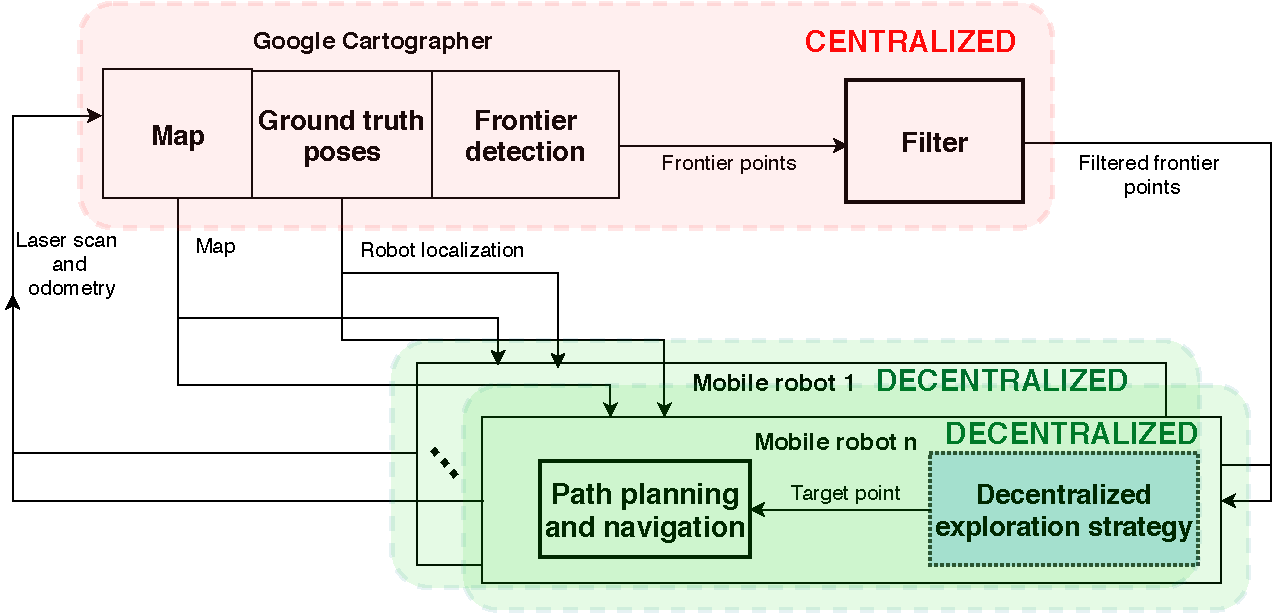
\includegraphics[width=1.0\columnwidth]{./pictures/diagram_exploration.pdf}
	\caption{Overall schematic diagram of the decentralized exploration and mapping process for $n$ robots in the simulator. Google Cartographer SLAM and filter module (highlighted in red) generate filtered frontier points that are (currently) the centralized part of exploration and mapping process. The exploration strategy, path planning and navigation module (highlighted green) are decentralized parts that generate $n$ outputs and create a common map.}
	\label{fig:exploration-strategy}
\end{figure}


\begin{algorithm}[b!]
	\While{Unexplored}{
		\If{Request}{
			Send position and current target point to the other mobile robots\;
		}
		\If{Robot has reached the previous target point}{
			Request positions and current target points from other mobile robots\;
			Calculate weight function\;
			Hungarian algorithm\;
			\textbf{return} Robot is assigned to frontier point\;
		}
	}
	\label{algorithm1}
	\caption{Decentralized strategy for multi-robot exploration.}
\end{algorithm}


Our decentralized strategy executes during the robot motion and there are steps for each robot to be executed (\textbf{Algorithm 1}). All frontier points are visible to all robots.
When a robot is assigned to a frontier point according to line 8 in \textbf{Algorithm 1}, the robot starts to follow the planned path and navigates to the target frontier point. At the moment when the robot reaches the target point (mission is over), a request is sent to other robots to get their positions and current target points. Calculated weight function are an input to Hungarian algorithm. 
The Hungarian algorithm is described in \cite{Kuhn1955} and tested in \cite{Kulich2015}. Initially, the Hungarian algorithm assumes that the number of frontier points is the same as the number of robots. Due to the fact that there are usually fewer robots than frontier points, virtual robots are added and then skipped during the process of assignment and exploration. 

The described process executes until the whole environment is explored and a complete  map of the environment is generated.

This approach is not only restricted to Google Cartographer SLAM and dense frontier detection, but may also be applied to different multi-robot systems. This strategy has resulted in improved behaviour in terms of exploration time compared to a state-of-the-art strategy in terms of exploration time. 



\section{3D exploration strategies}

\tp{Nije sasvim jasno u ovim svim pristupima da li koriste single robot ili multi robot, treba to negdje napisati.}
In contrast to 2D exploration and mapping strategies, mapping of large environments in 3D requires high memory and computational consumptions. 
Different autonomous 3D exploration strategies were proposed \st{so} that {\color{red}apply} 2D exploration tools \st{are used}  to three dimensions. In \cite{Joho2007}, Joho et al. presented an exploration strategy that extends the known 2D exploration strategies into the 3D space. Mapping is done using multi-level surface maps while a cost function takes
into account an expected information gain and a travel cost. 
Bachrach et
al. \cite{Bachrach2009} presented a solution for enabling a quadrotor helicopter to autonomously explore and map unstructured indoor environments. Authors used a 2D frontier-based exploration algorithm and set a fixed altitude for the helicopter during exploration.  

Dornhege and Kleiner \cite{Dornhege2013} used a frontier based method extended to 3D exploration. This method requires high computational effort and operating environment is limited to small workspaces. On the other hand, Maurovic et al. \cite{Maurovic2014} presented a 3D exploration strategy for a mobile robot equipped with a 3D laser scanner. This strategy ensures an online room detection algorithm focused on the room-by-room exploration keeping the memory and computational requirements low.

Priyasad et al. \cite{Priyasad2018} presented a point cloud based algorithm which can be used in a situation where the prior knowledge of the environment is highly inaccurate. The algorithm uses depth images to get a local map, which is expanded by searching for uncharted areas picking the next best
location to explore using a breadth first approach given a set of
constraints. The proposed algorithm exploits the maps in the 3D
space allowing the navigation system to perform effectively in uneven terrains. 

Next-best-view approach in the process of building 3D model of a real object used without any a priori information about the environment was described in \cite{VasquezGomez2014}. The algorithm determines each view to reconstruct an arbitrary object. Furthermore, authors proposed a method to deal with the uncertainty in sensor positioning.
Next-best-view approach for 3D exploration was presented by Bircher et. al. \cite{Bircher2016}. Authors presented a novel path planning algorithm for the autonomous exploration of an unknown area. The proposed planner finds the best branch in an online computed tree. The quality of the branch is determined by the amount of unmapped space that can be explored. The planner is capable of running online, onboard a robot with limited resources.

Baiming et al. \cite{Baiming2018} presented a new target points based trajectory planning algorithm to explore unknown space. The proposed method progressively plans long-term target point, intermediate target point, local target points, and local trajectory within real time constraint. By tracking the trajectory, robot can efficiently explore the unknown space while avoiding obstacles.

Zhu et al. \cite{Zhu2015} developed a vision-based tool that performs autonomous exploration using an MAV equipped with 3D sensors. A real time frontier based exploration strategy is used to build maps that are stored in the OctoMap format (Fig. \ref{fig:octomap}).

\begin{figure}[t!]
	\centering
	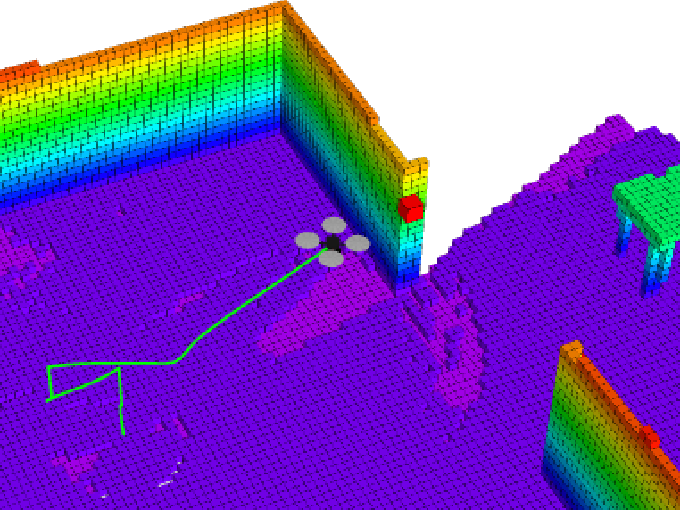
\includegraphics[width=1.0\columnwidth]{./pictures/octomap_and_drone.png}	
	\caption{UAV exploration in 3D environment. The colored voxels are 3D OctoMap representation and the green lines show the exploration trajectory \cite{Wang2019}.}
	\label{fig:octomap}
\end{figure}

Continuous cells are gathered into clusters and representative cells are chosen for each cluster. An evaluation function is used to choose the best representative cell and only state-changed space in the 3D map is processed in each iteration.
Authors in \cite{Senarathne2016} presented an alternative approach to 3D
exploration based on surface frontier voxels. The strategy focuses on seeking the expansion of mapped surfaces, instead of reducing unmapped voxels. 

Vutetakis in \cite{Vutetakis2019} proposed a novel strategy for inspecting
critical infrastructure autonomously using Micro Aerial Vehicles (MAV). In order to facilitate autonomous inspection capabilities, this strategy addresses the problem of autonomous MAV exploration and coverage of an unknown structure to acquire the spatial information necessary for the development of a high-fidelity 3D model of the structure. Key to this problem is to not only cover the entire structure, but also to minimize accumulative data errors during the exploration through direct planning of loop closures. 

Rocha et al. \cite{Rocha2005} dealt with 3D mapping by multiple robots using cubic cells for information storage. Authors presented a technique which is used for frontier-based exploration. At the beginning of the exploration an initial map is given to the robot, the robots update old map by new set of information \st{which calculate by measurement} {\color{red}obtained through sensing} and share their useful information with other robots. The process is repeated until the whole area is explored and mapped.

Wang et al. \cite{Wang2018} studied the problem of autonomous exploration in unknown indoor environments using mutual information to evaluate the information the robot would get at a certain location. Authors proposed a
sampling method that can get random sensing patches in free space. In order to to collect information with true values, each sensing patch is extended to informative locations. They combined it with Gaussian
Markov Random Fields (GMRF) to model the distribution of mutual information in environment.  Authors also proposed a utility function that can balance the path cost and the information gain the robot
would collect.

The 3D exploration problem using aerial vehicles within limited flight endurance was addressed by Wang et al. \cite{Wang2019}. Authors proposed an information potential field based method considering both the traveled cost and information-gain. The next-best-view point is chosen based on a multi-objective function which considers information of several candidate regions and the traveled path cost. The selected goal
attracts the robot while known obstacles form the repulsive
force repel the robot.



\begin{figure}[t!]
	\centering
	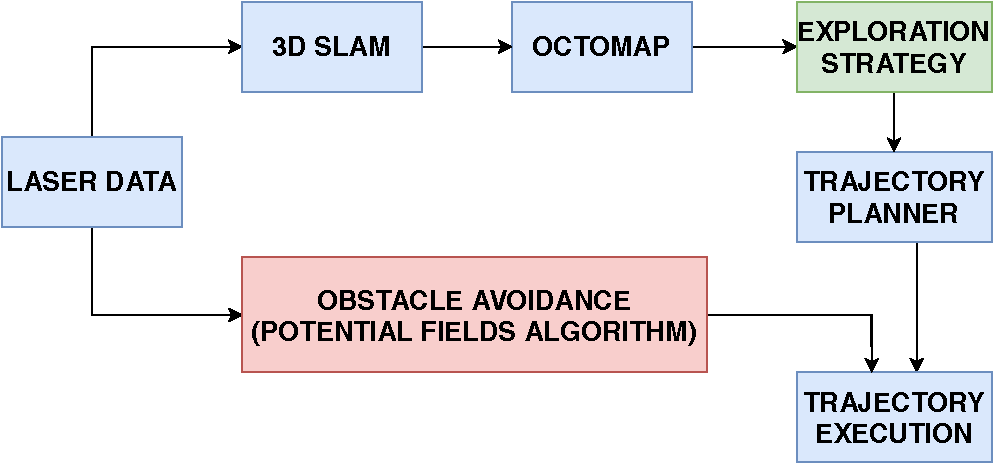
\includegraphics[width=1.0\columnwidth]{./pictures/3D_strategy.pdf}	
	\caption{Diagram of the implemented 3D exploration strategy.}
	\label{fig:3D_strategy}
\end{figure}


There are many algorithms to implement autonomous exploration as we described in the text above. Most of the algorithms are dependent on prior knowledge of the environment and apriori maps. Although
they are effective in some scenarios, these algorithms fail to
perform when the environment has been subjected to changes
that might invalidate the prior map. There are also algorithms implemented to deal with single robot exploration and mapping. Motivated by mentioned facts, we studied the problem of autonomous building exploration with purpose of fire detection. 
Besides
the localization and mapping of an unknown area, laser data is used for an OctoMap generation (Fig. \ref{fig:3D_strategy}). Google Cartographer SLAM crates a map in which a robot gets a goal point and using OctoMap generate trajectory and execute it. Obstacle avoidance is also considered in our work.
\begin{figure}
	\centering
	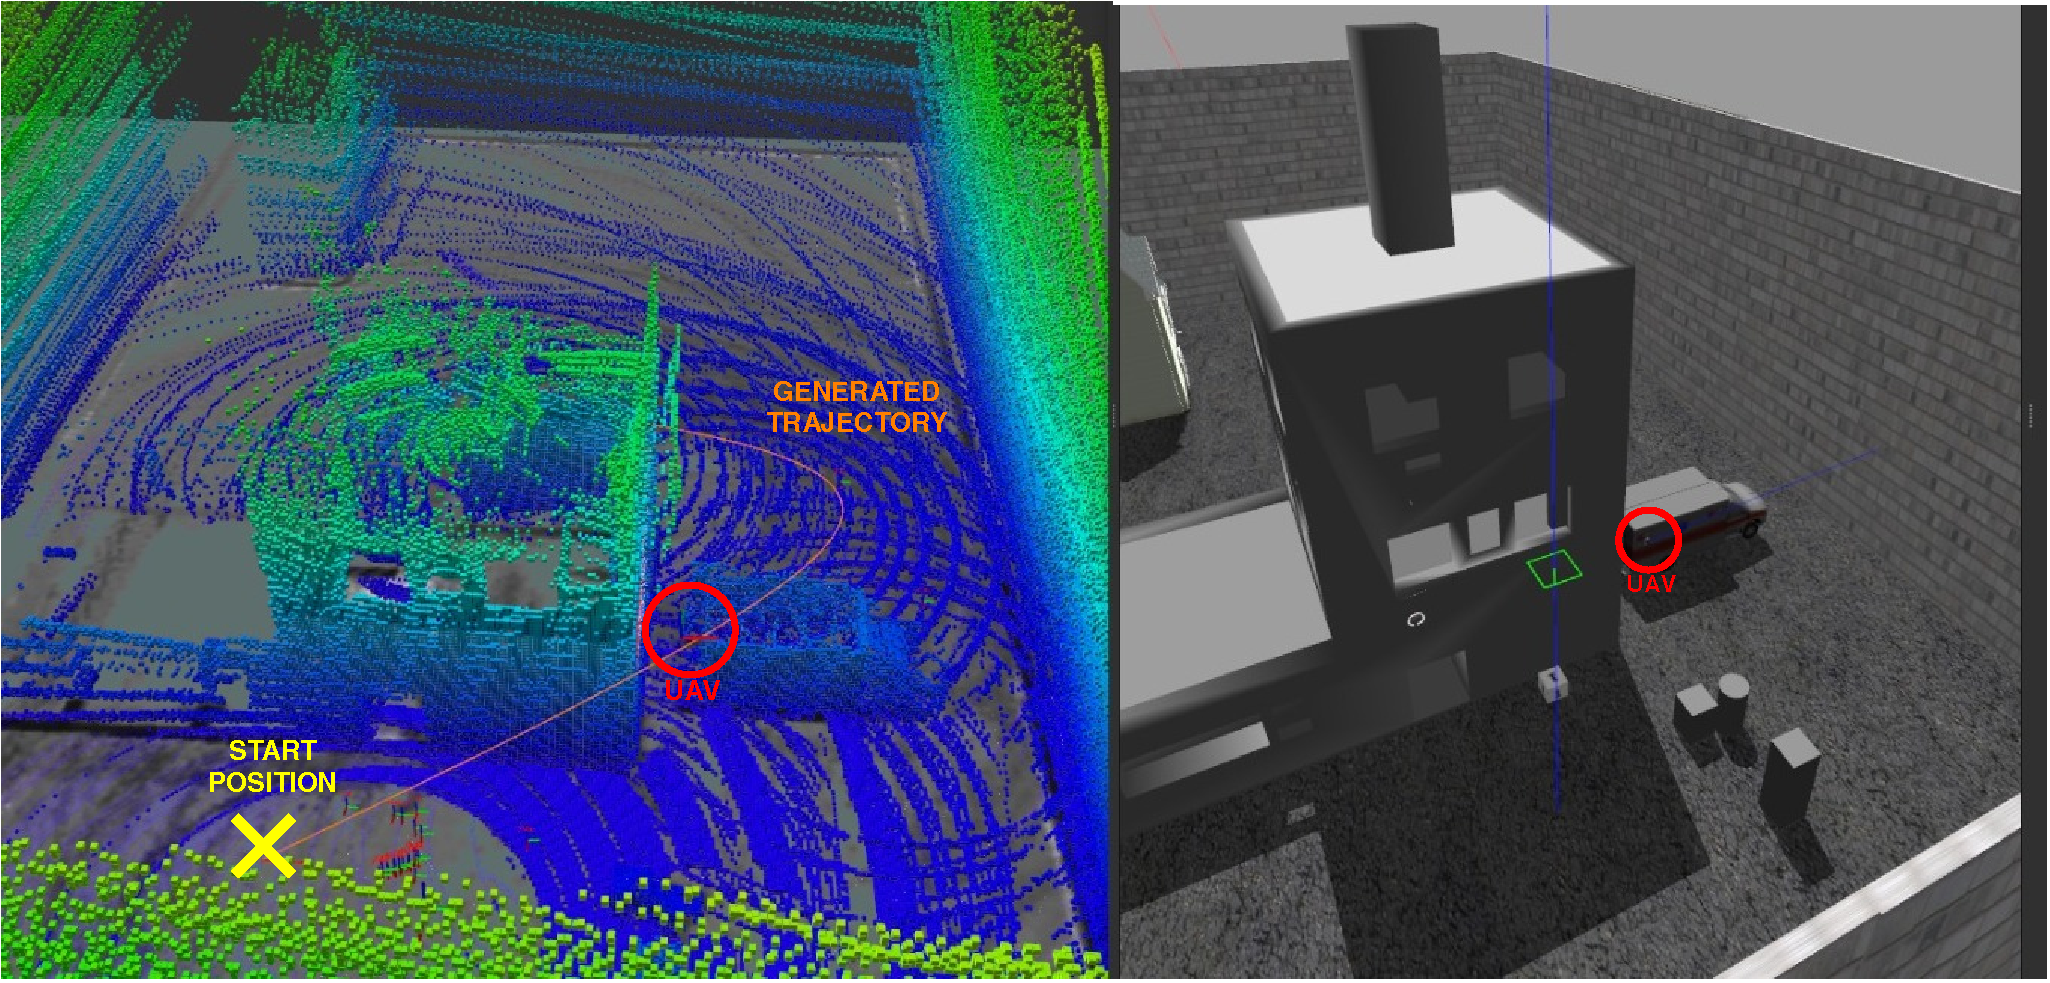
\includegraphics[width=1.0\columnwidth]{./pictures/rviz_gazebo.pdf}	
	\caption{}
	\label{fig:rviz_gazebo}
\end{figure}
\section{Conclusion and future work} \label{sec:conclusion}

The problem of autonomous environment exploration is complex, because it includes the control of a robot, an environment scanning with a 3D sensor, creating a volumetric consistent scene in a common coordinate system from multiple views, the computation of next view points to provide efficiently full coverage of the scene, an elimination of an 
occlusion under the constraint of minimizing the total
path length between these points. 

In this paper, a brief overview of the exploration strategies is given. 
%A modular approach to autonomous decentralized multi-robot exploration and mapping was presented. Even though the strategy achieved our expectations, the algorithm is open towards improving. Future research should consider decentralized map creating. Also, a significant improvement to this strategy would be a simpler simulator, that would allow for simulation of more robots.

Another research direction can be an extension to the 3D space including multi aerial vehicles (MAVs).  algorithm to cope with a limited communication range of the mobile robots. Future work should also consider a multi-robot system which uses a (not fully) connected communication graph. Finally, we would like to take into consideration scenarios in which the robots may fail as well as time-varying environment scenarios.

This paper presents a solution to autonomously explore 3D environment without requiring an initial map or goal point. Octomap itself is able to handle dynamic environments by updating the map which makes the
algorithm works well in dynamic environment as the point
cloud is extracted from it.

This work is a stepping stone for new research in multi-robot exploration algorithms and its decentralization. There is also huge opportunity in 3D mapping and exploration, since ...

%%%%%%%%%%%%%%%%%%%%%%%%%%%%%%%%%%%%%%%%%%%%%%%%%%%%%%%%%%%%%%%%%%%%%%%%%%%%%%%%
%\section*{APPENDIX} \label{sec:appendix}
%In this section rotating body dynamics with variations in center of gravity is derived.
General form of Euler-Lagrange dynamics for a rotating rigid body on SE(3) configuration manifold in the body-fixed frame as presented in \cite{LeeModel}:

\begin{gather}
	\frac{d}{dt} \left( \frac{\partial \La}{\partial \mb{\Omega}} \right)
	+ \mb{\Omega} \times \frac{\partial \La}{\partial \mb{\Omega}} 
	+ \textbf{v} \times \frac{\partial \La}{\partial \textbf{v}} 
	+ \sum_{i=1}^{3} \textbf{r}_i \times \frac{\partial \La}{\partial \textbf{r}_i} = 0 \label{general1}\\
	\frac{d}{dt} \left( \frac{\partial \La}{\partial \textbf{v}} \right)
	+ \mb{\Omega} \times \frac{\partial \La}{\partial \textbf{v}} 
	- \text{R}^T \frac{\partial \La}{\partial x} = 0 \label{general2}
\end{gather}
For the proposed UAV with variations in CoG the Lagrangian is:

\begin{gather}
\begin{align}
\begin{split}
	\La(\text{R},x,\mb{\Omega},\textbf{v}) &= \frac{1}{2}\mb{\Omega}^T\text{J}\mb{\Omega} \,+\, m \mb{\Omega}^T \reallywidehat{\textbf{r}}_{CoG}\textbf{v} \\
	\, &+\, \frac{1}{2}m\textbf{v}^T\textbf{v} \,-\, U(\text{R},\textbf{x}) \, ,
\end{split}
\end{align}
\end{gather}
where $U(\text{R}, \textbf{x})$ is the potential energy. It is important to note that \text{J} and $\textbf{r}_{CoG}$ are variable over time. \\
%Lagrangian derivatives needed for the general form equations \ref{general1} and \ref{general2} are:
%\begin{gather}
%	\frac{\partial \La}{\partial \mb{\Omega}} = \text{J}\mb{\Omega} + m \reallywidehat{\textbf{r}}_{CoG}\textbf{v} \label{d1}\\ 
%	\frac{d}{dt} \left( \frac{\partial \La}{\partial \mb{\Omega}} \right) = \dot{\text{J}} \mb{\Omega} + \text{J} \dot{\mb{\Omega}} + m \dot{\textbf{r}}_{CoG} \times \textbf{v} + m \textbf{r}_{CoG} \times \dot{\textbf{v}} \label{d2}\\ 
%	\frac{\partial \La}{\partial \textbf{v}} = m\textbf{v} - m\textbf{r}_{CoG} \times \mb{\Omega} \label{d3}\\ 
%	\frac{d}{dt} \left( \frac{\partial \La}{\partial \textbf{v}} \right) = m\dot{\textbf{v}} - m\dot{\textbf{r}}_{CoG} \times \mb{\Omega} - m \textbf{r}_{CoG} \times \dot{\mb{\Omega}} \label{d4}
%\end{gather}
It is of interest to transfer rotation and translation dynamics in the inertial frame. This can be done using the following relations:
\begin{gather}
	\textbf{v} = \text{R}^T \dot{x} \label{inertial1}\\
	\dot{\textbf{v}} = \text{R}^T \ddot{\textbf{x}} - \mb{\Omega} \times (\, \text{R}^T \dot{\textbf{x}} \,) \label{inertial2} \\
	\textbf{r}_{CoG} = \text{R}^T(\, \textbf{x}_{CoG} - \textbf{x} \,) \label{inertial3} \\
	\dot{\textbf{r}}_{CoG} = \text{R}^T(\, \dot{\textbf{x}}_{CoG} - \dot{\textbf{x}} \,) - \reallywidehat{\mb{\Omega}}\text{R}^T(\, \textbf{x}_{CoG} - \textbf{x} \,) \label{inertial4}
\end{gather}
After computing Lagrangian derivatives, plugging them in \ref{general1}, \ref{general2} and using \ref{inertial1}, \ref{inertial2} as velocity and acceleration transformations to the inertial frame the following equations are obtained:
\begin{gather}
\label{complete_model1}
\begin{align}
	\begin{split}
		\text{J}\dot{\mb{\Omega}} &+ m \textbf{r}_{CoG} \times \text{R}^T \ddot{\textbf{x}} + \mb{\Omega} \times \text{J}\mb{\Omega} \\
		&+ \dot{\text{J}} \mb{\Omega} + m \dot{\textbf{r}}_{CoG} \times \text{R}^T \dot{\textbf{x}} + \sum_{i=1}^{3} \textbf{r}_i \times \frac{\partial \La}{\partial \textbf{r}_i} = 0
	\end{split}
\end{align}
\end{gather}
\begin{gather}
\label{complete_model2}
\begin{align}
	\begin{split}
		m \ddot{\textbf{x}} & - m \text{R} \,(\, \textbf{r}_{CoG} \times \dot{\mb{\Omega}} \,) - m \text{R} \,[\, \mb{\Omega} \times (\, \textbf{r}_{CoG} \times \mb{\Omega} \,) \,] \\
		&- m \text{R} \,(\, \dot{\textbf{r}}_{CoG} \times \mb{\Omega} \,) + \frac{\partial U(\text{R},\textbf{x})}{\partial \textbf{x}} = 0
	\end{split}
\end{align}
\end{gather}
Finally, CoG transforms \ref{inertial3} and \ref{inertial4} are included along with forces and moments acting in the body-fixed frame which gives the following model dynamics:
\begin{gather}
\begin{align}
	\begin{split}
		 \text{J}\dot{\mb{\Omega}} & + m \textbf{r}_{CoG} \times \text{R}^T\ddot{\textbf{x}} + \mb{\Omega} \times \text{J}\mb{\Omega}  \\
		 & - m (\, \mb{\Omega} \times \textbf{r}_{CoG} \,) \times \text{R}^T \dot{\textbf{x}} \\
		 & + \dot{\text{J}}\mb{\Omega} + m \, \reallywidehat{R^T (\, \dot{\textbf{x}}_{CoG} - \dot{\textbf{x}} \,)} \, R^T\dot{\textbf{x}} = \textbf{M}
	\end{split}
\end{align}
\end{gather}
\begin{gather}
\begin{align}
	\begin{split}
		m \ddot{\textbf{x}} & - m \text{R} \,(\, \textbf{r}_{CoG} \times \dot{\mb{\Omega}} \,) + m g\textbf{e}_3 \\
		& - m \text{R} \, \reallywidehat{ \text{R}^T (\, \dot{\textbf{x}}_{CoG} - \dot{\textbf{x}} \,) } \, \mb{\Omega}  = f\text{R}\textbf{e}_3
	\end{split}
\end{align}
\end{gather}
\noindent Please note that \textit{wide hat} is the same operator previously defined in \eqref{eqn:hat}.

%Appendixes should appear before the acknowledgment.

%\section*{ACKNOWLEDGMENT}



%%%%%%%%%%%%%%%%%%%%%%%%%%%%%%%%%%%%%%%%%%%%%%%%%%%%%%%%%%%%%%%%%%%%%%%%%%%%%%%%

%\nocite{*}
\bibliographystyle{ieeetr}

\bibliography{bibliography/Mendeley}

\end{document}
